% Fully connected neural network
% Author: Izaak Neutelings (September 2021) 
% https://tikz.net/neural_networks/

\documentclass[border=3pt,tikz]{standalone}
% Fully connected neural network
% Author: Izaak Neutelings (September 2021) 
% Adapted from https://tikz.net/neural_networks/

\usepackage{neuralnetwork}
\usepackage{amsmath} % for aligned
\usepackage{tikz}
\usepackage{listofitems} % for \readlist to create arrays
\usetikzlibrary{arrows.meta} % for arrow size
\usepackage[outline]{contour} % glow around text
\contourlength{1.4pt}

\tikzset{>=latex} % for LaTeX arrow head
\usepackage{xcolor}
\definecolor{orblue}{RGB}{0, 90, 169} 
\definecolor{logred}{RGB}{185, 15, 34}
\definecolor{tugreen}{RGB}{127, 171, 22}

\tikzstyle{node}=[thick,circle,draw=orblue,minimum size=22,inner sep=0.5,outer sep=0.6]
\tikzstyle{node in}=[node,green!20!black,draw=tugreen!30!black,fill=tugreen!30]
\tikzstyle{node hidden}=[node,blue!20!black,draw=orblue!30!black,fill=orblue!30]
\tikzstyle{node out}=[node,red!20!black,draw=logred!30!black,fill=logred!30]
\tikzstyle{connect}=[thick,black] %,line cap=round
\tikzstyle{connect arrow}=[-{Latex[length=4,width=3.5]},thick,black,shorten <=0.5,shorten >=1]
\tikzset{ % node styles, numbered for easy mapping with \nstyle
  node 1/.style={node in},
  node 2/.style={node hidden},
  node 3/.style={node out},
}
\def\nstyle{int(\lay<\Nnodlen?min(2,\lay):3)} % map layer number onto 1, 2, or 3

\begin{document}
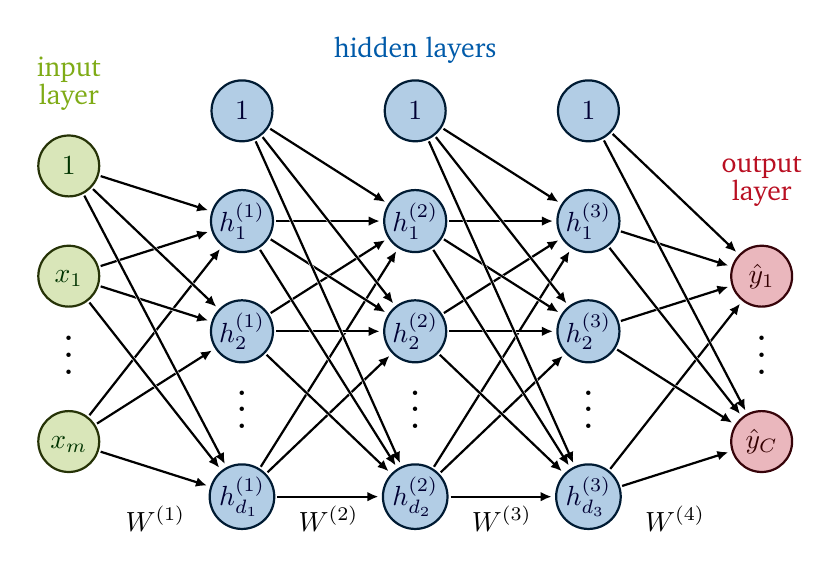
\begin{tikzpicture}[x=2.2cm,y=1.4cm]
  \message{^^JNeural network, shifted}
  \readlist\Nnod{2,3,3,3,2} % array of number of nodes per layer
  \readlist\Nstr{m,d_1,d_2,d_3,C} % array of string number of nodes per layer
  \readlist\Cstr{\strut x,h^{(\prev)},h^{(\prev)},h^{(\prev)},\hat{y}} % array of coefficient symbol per layer
  \def\yshift{0.5} % shift last node for dots
  
  \message{^^J  Layer}
  \foreachitem \N \in \Nnod{ % loop over layers
    \def\lay{\Ncnt} % alias of index of current layer
    \pgfmathsetmacro\prev{int(\Ncnt-1)} % number of previous layer
    \message{\lay,}
    \foreach \i [evaluate={\c=int(\i==\N); \y=\N/2-\i-\c*\yshift;
                 \index=(\i<\N?int(\i):"\Nstr[\lay]");
                 \x=\lay; \n=\nstyle;}] in {0,...,\N}{ % loop over nodes
        % NODES
        % \ifnum\lay=1 % first layer
        %   \ifnum\i=0 % first node = input bias
        %     \node[node \n] (N\lay-\i) at (\x,\y) {$1$};
        %   \else % other nodes
        %     \node[node \n] (N\lay-\i) at (\x,\y) {$\Cstr[\lay]_{\index}$};
        %   \fi
        % \else
        \ifnum\lay=\Nnodlen % last layer
          \ifnum\i>0 % no bias
            \node[node \n] (N\lay-\i) at (\x,\y) {$\Cstr[\lay]_{\index}$};
          \fi
        \else % other layers
          \ifnum\i=0 % first node = input bias
            \node[node \n] (N\lay-\i) at (\x,\y) {$1$};
          \else % other nodes
            \node[node \n] (N\lay-\i) at (\x,\y) {$\Cstr[\lay]_{\index}$};
          \fi
        \fi
        % CONNECTIONS
        \ifnum\lay>1
          \ifnum\i>0% connect to previous layer
              \foreach \j in {0,...,\Nnod[\prev]}{ % loop over nodes in previous layer
                \draw[connect,white,line width=1.2] (N\prev-\j) -- (N\lay-\i);
                \draw[connect arrow] (N\prev-\j) -- (N\lay-\i);
                %\draw[connect] (N\prev-\j.0) -- (N\lay-\i.180); % connect to left
              }
          \fi
        \fi % else: nothing to connect first layer
      
    }
    \path (N\lay-\N) --++ (0,1+\yshift) node[midway,scale=1.5] {$\vdots$};
  }

  % LABELS
  {\fontfamily{bch}\selectfont
  \node[above=5,align=center,tugreen!100] at (N1-0.90) { input\\[-0.2em]layer};
  \node[above=2,align=center,orblue!100] at (N3-0.90) {hidden layers};
  \node[above=10,align=center,logred!100] at (N\Nnodlen-1.90) {output\\[-0.2em]layer};
  }
  \node[below=0,align=center,black!100] at (1.5,-2) {${W}^{(1)}$};
  \node[below=0,align=center,black!100] at (2.5,-2) {${W}^{(2)}$};
  \node[below=0,align=center,black!100] at (3.5,-2) {${W}^{(3)}$};
  \node[below=0,align=center,black!100] at (4.5,-2) {${W}^{(4)}$};
  
\end{tikzpicture}
\end{document}